\section{Systembeskrivelse}
Der ønskes, som tidligere nævnt, at udvikle et system, der har til formål at aflaste musklerne omkring knæleddet under udførelse af en statisk squat-bevægelse ved brug af et exoskelet. Dette gøres for at aflaste patienterne med henblik på at kunne undgå kørestol i tidlige stadier af ALS. Systemet skal kunne opsamle signaler fra lårmusklerne; quadriceps og hamstring. Disse signaler skal behandles og omsættes til aktivitet i en prototype af et exoskelet, som skal udføre en tilsvarende bevægelse, men også have mulighed for forstærkning af signalet, så mindre muskelkraft også vil kunne udløse denne bevægelse. Ud over aktiviteten i musklerne skal exoskelettet kunne begrænse bevægelse i visse retninger, så det herved er muligt at rette leddets position, hvis dette bevæger sig uønsket\fxnote{har vi snakket om dette?}. Af denne grund skal systemet være i stand til at måle muskelaktivitet i quadriceps og hamstring samt den aktuelle vinkel i knæleddet. Derudover skal systemet være brugervenligt ved at være kompakt, mobilt og ikke generende over for brugeren.

\subsection{Krav til systemet} 
\begin{itemize}
\item Systemet skal registrere muskelaktivitet og ledvinkler
\item Systemet skal kunne overføre data trådløst til en computer
\item Systemet skal kunne udmundes(bedre ord?) i en prototype af et exoskelet
\item Systemet skal være batteridrevet
\item Systemet skal være sikkert og ikke til gene for brugeren
\item Systemet skal kunne indikere, hvis der ikke er strøm nok til at virke optimalt \fxnote{er dette et vigtigt punkt?}
\item Systemet skal kunne give feedback og derved sørge for, at brugeren befinder sig inden for følgende specifikationer:\fxnote{igen: har vi snakket om dette?}
\begin{itemize}
\item XX antal grader?
\item XX antal grader?
\end{itemize}
\end{itemize}

\fxnote{Punkterne står virkelig tæt på teksten - kan vi ændre på det?}

\subsection{Blokdiagram}\fxnote{ændr feedback til prototype, tilføj måske patienten}
\begin{figure}[H]
\centering
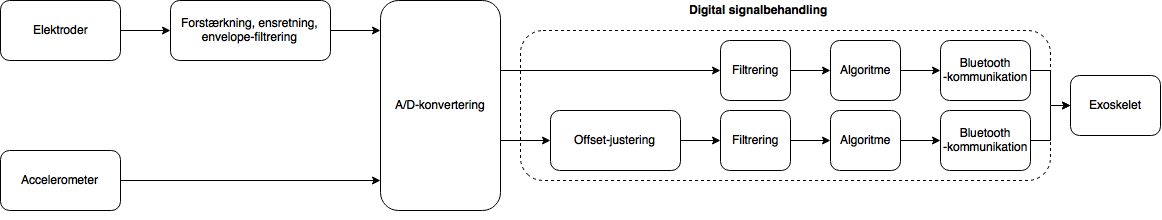
\includegraphics[width=0.4\textwidth]{figures/blokdiagram.png}
\caption{Systemets opbygning.}
\label{fig:blokdiagram}
\end{figure}

%I dette projekt er der valgt at udarbejde en prototype, som har til formål at sørge for at knæledddet forbliver inden for en bestemt position. 
I dette projekt er der valgt at udarbejde en prototype, som har til formål at bøje knæleddet, når lårets muskler kontraherer. Opbygningen af systemet fremgår af \autoref{fig:blokdiagram}. Der anvendes to sensorer, EMG og accelerometer, til at opsamle biologiske signaler, For at registrere muskelaktivitet anvendes en EMG-sensor og en EMG-forstærker, der har til formål at forstærke den muskelaktivitet, der opsamles. Accelerometeret anvendes for at give systemet et input om, knæleddet vinkles  under udøvelsen af en statisk squat. Det opsamlede signal sendes herefter videre til den digitale del af systemet, hvilket er bestående af et Bluetooth Low Energy Pioneer kit (CY8CKIT-042-BLE), som opfanger de biologiske signaler og overfører dem trådløst til en CySmartUSB BLE Dongle sat i en computer, som kan kommunikere med prototypen af exoskelettet i LEGO Mindstorms. 


